\chapter{Espécies químicas naturais e sintéticas}\label{ch:g10:chemical-species}

Uma colherada de sorvete de baunilha. O sabor pode vir das vagens pretas
de uma orquídea tropical, colhidas, curadas e mergulhadas em álcool
durante meses; ou pode vir de uma fábrica que produz o aroma a partir da
polpa de madeira ou do petróleo. Prove os dois lado a lado e o sabor
principal é o mesmo --- por uma boa razão: a \omterm{def:g7:atoms-and-molecules:molecule}{molécula} que tem gosto de
baunilha, a vanilina, é exatamente a mesma \omterm{def:g7:atoms-and-molecules:molecule}{molécula}, seja qual for o
modo como foi obtida. Este capítulo mostra como os químicos tiram uma
espécie de uma planta, como a fabricam e como verificam que o que têm é
mesmo o que pensam ter.

\begin{recall}
Uma \omterm{def:g6:pure-substances-and-mixtures:species}{espécie química} é um tipo determinado de substância; uma \omterm{def:g6:pure-substances-and-mixtures:pure-substance}{substância
pura} contém uma única espécie e tem constantes fixas, como as
temperaturas de fusão e de ebulição
(\cref{ch:g6:pure-substances-and-mixtures}). Os líquidos são \omterm{def:g6:solutions-and-solubility:miscible}{miscíveis}
ou \omterm{def:g6:solutions-and-solubility:miscible}{imiscíveis}, e cada \omterm{def:g6:solutions-and-solubility:solute}{soluto} tem a sua própria \omterm{def:g6:solutions-and-solubility:solubility}{solubilidade} em cada
\omterm{def:g6:solutions-and-solubility:solute}{solvente} (\cref{ch:g6:solutions-and-solubility}). A \omterm{def:g7:identifying-substances:chromatography}{cromatografia em
papel} separa os corantes de uma \omterm{def:g6:pure-substances-and-mixtures:mixture}{mistura}
(\cref{ch:g7:identifying-substances}).
\end{recall}

\begin{omfigure}
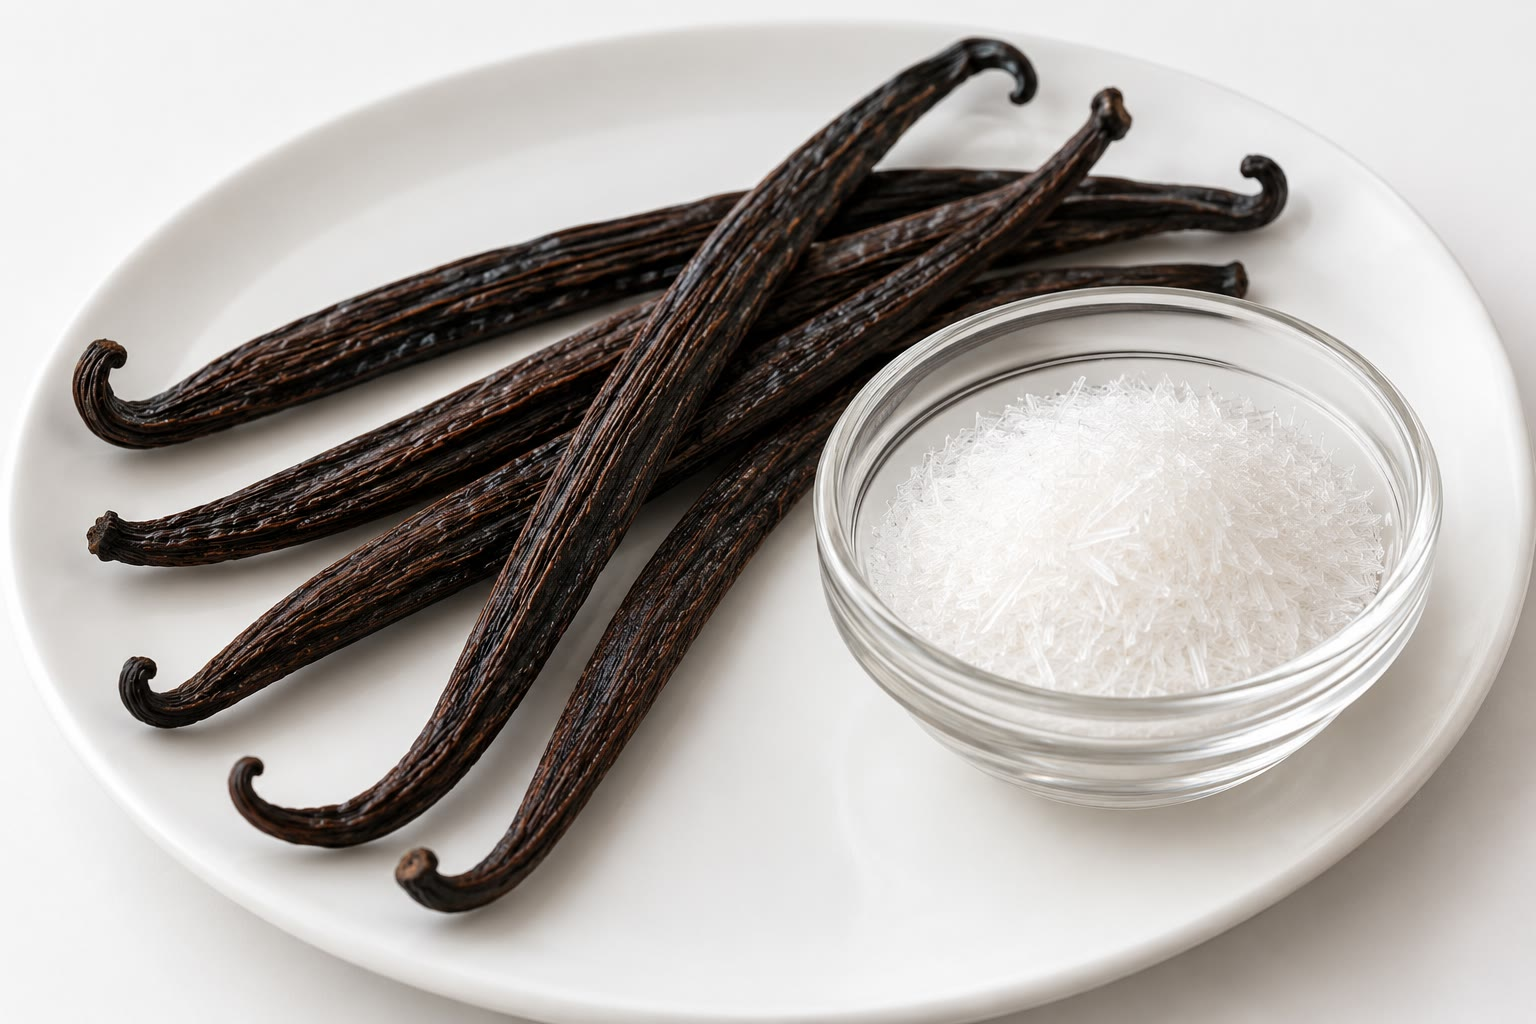
\includegraphics[width=0.55\linewidth]{images/book1/ai/g10-vanilla.jpg}

{\small Vagens de baunilha e cristais brancos de vanilina: a mesma
\omterm{def:g7:atoms-and-molecules:molecule}{molécula}, vinda de uma planta ou de uma fábrica.}
\end{omfigure}

\section{Espécies naturais e sintéticas}

\begin{definition}[Espécies naturais e sintéticas]\label{def:g10:chemical-species:natural}
Uma \emph{espécie natural}\index{especie natural@espécie natural} é uma \omterm{def:g6:pure-substances-and-mixtures:species}{espécie química}
produzida por um ser vivo ou encontrada como tal na natureza. Uma
\emph{espécie sintética}\index{especie sintetica@espécie sintética} é produzida pelos
químicos a partir de outras espécies, por meio de \omterm{def:g7:chemical-reactions:reaction}{reações químicas}. Uma
espécie sintética pode ser idêntica a uma espécie natural (a vanilina
sintética) ou não ter equivalente na natureza (a maioria dos remédios e
dos \omterm{def:g8:plastics:plastic}{plásticos}).
\end{definition}

\begin{proposition}[Mesma espécie, mesmas propriedades]\label{prop:g10:chemical-species:same}
Uma \omterm{def:g6:pure-substances-and-mixtures:species}{espécie química} tem as mesmas propriedades seja qual for a sua
origem: a vanilina produzida numa fábrica e a vanilina extraída de uma
vagem têm a mesma fórmula, o mesmo ponto de fusão, o mesmo cheiro. O que
pode ser diferente é o que vem junto com ela: um extrato natural é uma
\omterm{def:g6:pure-substances-and-mixtures:mixture}{mistura}, com muitas outras espécies que mudam o seu sabor.
\end{proposition}

\begin{history}[Da casca do salgueiro à aspirina, 1828--1899]
Durante séculos, a casca do salgueiro foi mascada contra a febre e a dor.
Em 1828, um químico extraiu dela a espécie ativa, a salicina; os
químicos a transformaram depois em ácido salicílico, que funciona mas
irrita o estômago. Em 1897, numa empresa de corantes e medicamentos,
Felix Hoffmann produziu a partir do ácido salicílico uma \omterm{def:g10:chemical-species:natural}{espécie
sintética} mais suave: o ácido acetilsalicílico, vendido a partir de 1899
com o nome de aspirina. A aspirina não tem fonte natural: ela é uma
espécie puramente sintética.
\end{history}

\section{Extrair uma espécie}

\begin{definition}[Extração e extração líquido--líquido]\label{def:g10:chemical-species:extraction}
Uma \emph{extração}\index{extracao@extração} retira uma \omterm{def:g6:pure-substances-and-mixtures:species}{espécie química} do
material que a contém, em geral dissolvendo-a num \omterm{def:g6:solutions-and-solubility:solute}{solvente} bem
escolhido. Numa \emph{extração líquido--líquido}\index{extracao liquido--liquido@extração líquido--líquido},
uma espécie dissolvida num líquido é transferida para um segundo líquido, \omterm{def:g6:solutions-and-solubility:miscible}{imiscível} com o primeiro, no qual ela \omterm{def:g2:mixing-and-dissolving:dissolve}{se dissolve}
melhor; os dois líquidos são depois separados num funil de separação.
\end{definition}

\begin{example}[Extrações do dia a dia]\label{ex:g10:chemical-species:everyday}
Fazer chá é uma \omterm{def:g10:chemical-species:extraction}{extração} com água quente (infusão); deixar vagens de
baunilha de molho no álcool é uma \omterm{def:g10:chemical-species:extraction}{extração} com etanol (maceração);
ferver legumes para fazer um caldo é outra (decocção).
\end{example}


\begin{definition}[Destilação e hidrodestilação]\label{def:g10:chemical-species:distillation}
Uma \emph{destilação}\index{destilacao@destilação} aquece uma \omterm{def:g6:pure-substances-and-mixtures:mixture}{mistura} líquida até a
ebulição, faz o vapor voltar a ser líquido num condensador resfriado por
água corrente e recolhe esse líquido, o destilado. Uma
\emph{hidrodestilação}\index{hidrodestilacao@hidrodestilação} ferve um material vegetal
na água: o vapor de água arrasta as espécies perfumadas da planta, que
se separam da água no destilado na forma de uma camada oleosa, o óleo
essencial.
\end{definition}

\begin{omfigure}
\begin{tikzpicture}[font=\small, scale=0.95]
  \pic[transform shape] at (0,0) {heatingmantle};
  \pic[transform shape] at (0,0) {rbflask={0.55}{omWater!70}};
  \foreach \x/\y in {-0.45/0.35,-0.1/0.55,0.3/0.3,0.5/0.7,-0.6/0.75,0.1/0.9,-0.25/0.2}
    \fill[green!45!black!70] (\x,\y) ellipse (0.09 and 0.04);
  \pic[transform shape] (s) at (0,3.0) {stillhead};
  \pic[transform shape] at ($(s-top)+(0,-0.75)$) {thermometer};
  \pic[transform shape, rotate=-20] (c) at (s-arm) {liebig={3.2}};
  \coordinate (cend) at ($(s-arm)+(-20:3.2)$);
  \pic[transform shape] (a) at (cend) {adapter};
  \pic[transform shape] at ($(a-tip)+(0,-2.3)$) {erlenmeyer={0.18}{omWater!70}};
  \fill[yellow!60!orange!60] ($(a-tip)+(-0.827,-2.3+0.47)$) -- ($(a-tip)+(0.827,-2.3+0.47)$) -- ($(a-tip)+(0.779,-2.3+0.6)$) -- ($(a-tip)+(-0.779,-2.3+0.6)$) -- cycle;
  \draw[<-, omProp, thick] (-0.55,0.55) -- (-2.2,0.9) node[left, text=black, align=right]
    {água e\\ flores de lavanda};
  \draw[<-, omProp, thick] (1.35,-0.6) -- (2.2,-1.1) node[right, text=black]
    {manta de aquecimento};
  \draw[<-, omProp, thick] (0.1,4.2) -- (-1.2,4.6) node[left, text=black] {termômetro};
  \draw[<-, omProp, thick] ($(s-arm)+(-20:1.6)+(0,0.32)$) -- ++(0.6,1.0) node[above, text=black]
    {condensador, resfriado por água corrente};
  \draw[<-, omProp, thick] ($(a-tip)+(0.4,-1.88)$) -- ++(1.1,0.2) node[right, text=black, align=left]
    {destilado: óleo essencial\\ flutuando sobre a água};
\end{tikzpicture}

{\small \omterm{def:g10:chemical-species:distillation}{Hidrodestilação} da lavanda. O vapor de água arrasta o óleo
essencial até o condensador; o destilado se separa numa fina camada de
óleo sobre a água.}
\end{omfigure}

\begin{method}[Escolher um solvente de extração]\label{met:g10:chemical-species:solvent}
Para uma \omterm{def:g10:chemical-species:extraction}{extração líquido--líquido} de uma espécie a partir da água, o
\omterm{def:g6:solutions-and-solubility:solute}{solvente} deve:
\begin{enumerate}
  \item \omterm{def:g2:mixing-and-dissolving:dissolve}{dissolver} a espécie muito melhor do que a água;
  \item ser \omterm{def:g6:solutions-and-solubility:miscible}{imiscível} com a água, para que se formem duas camadas;
  \item ser o menos perigoso possível, e fácil de retirar depois (uma
        temperatura de ebulição baixa permite fazê-lo evaporar).
\end{enumerate}
A camada que fica em cima é decidida pelas densidades: o líquido menos
denso flutua.
\end{method}

\begin{example}[Solventes para o óleo de lavanda]\label{ex:g10:chemical-species:table}
% ledger: rho:cyclohexane, bp:cyclohexane, rho:ethyl-acetate, bp:ethyl-acetate, rho:CH2Cl2, bp:CH2Cl2, rho:ethanol, bp:ethanol, sol:linalool
O linalol, a principal espécie do óleo de lavanda, só \omterm{def:g2:mixing-and-dissolving:dissolve}{se dissolve} até
\qty{1.6}{g/L} na água, mas muito bem nos \omterm{def:g6:solutions-and-solubility:solute}{solventes} abaixo:
\begin{center}
\small
\begin{tabular}{lccll}
\hline
\omterm{def:g6:solutions-and-solubility:solute}{solvente} & massa de \qty{1}{mL} & ferve a & com a água & principais perigos \\
\hline
ciclo-hexano & \qty{0.78}{g} & \qty{81}{\celsius} & \omterm{def:g6:solutions-and-solubility:miscible}{imiscível} & inflamável, nocivo \\
etanoato de etila & \qty{0.90}{g} & \qty{77}{\celsius} & \omterm{def:g6:solutions-and-solubility:miscible}{imiscível} & inflamável, irritante \\
diclorometano & \qty{1.33}{g} & \qty{40}{\celsius} & \omterm{def:g6:solutions-and-solubility:miscible}{imiscível} & suspeito de ser cancerígeno \\
etanol & \qty{0.79}{g} & \qty{78}{\celsius} & \omterm{def:g6:solutions-and-solubility:miscible}{miscível} & inflamável \\
\hline
\end{tabular}
\end{center}
O etanol não pode ser usado: ele se mistura com a água e não se formam
camadas. Com o ciclo-hexano ou o etanoato de etila, a camada de \omterm{def:g6:solutions-and-solubility:solute}{solvente}
fica em cima; com o diclorometano, embaixo.
\end{example}

\begin{omfigure}
\begin{tikzpicture}[font=\small, scale=1.2]
  \pic[transform shape] at (0,0) {sepfunnel={omWater!70}{yellow!35!orange!35}};
  \draw[<-, omProp, thick] (0.55,2.1) -- (1.6,2.4) node[right, text=black, align=left]
    {ciclo-hexano e o óleo\\ (menos denso, em cima)};
  \draw[<-, omProp, thick] (0.55,1.3) -- (1.6,1.2) node[right, text=black, align=left]
    {água, escoada\\ pela torneira};
  \draw[<-, omProp, thick] (0.25,0.52) -- (1.6,0.4) node[right, text=black] {torneira};
\end{tikzpicture}

{\small Um funil de separação depois de agitado e deixado em repouso: o
óleo passou para o ciclo-hexano, em cima.}
\end{omfigure}

\begin{safety}{\ghs[0.8cm]{GHS02}\ghs[0.8cm]{GHS07}\ghs[0.8cm]{GHS08}\ghs[0.8cm]{GHS09}}
% ledger: ghs:cyclohexane
Ciclo-hexano: altamente inflamável (GHS02); pode ser mortal se ingerido
e penetrar nas vias respiratórias, provoca irritação da pele e
sonolência (GHS07, GHS08); muito tóxico para os organismos aquáticos
(GHS09). Usado numa capela de exaustão, longe de chamas.
\end{safety}

\section{A cromatografia em camada delgada}

\begin{definition}[Cromatografia em camada delgada]\label{def:g10:chemical-species:tlc}
A \emph{cromatografia em camada delgada}\index{cromatografia em camada delgada}
(CCD) separa as espécies de uma \omterm{def:g6:pure-substances-and-mixtures:mixture}{mistura} numa placa coberta por uma fina
camada de um pó branco fino, a \emph{fase estacionária}\index{fase estacionaria@fase estacionária}.
Pequenas manchas das amostras são postas sobre uma linha
a lápis perto da base; a placa fica de pé, numa cuba fechada, num pouco
de \omterm{def:g6:solutions-and-solubility:solute}{solvente}, o \emph{eluente}\index{eluente}, que sobe pela placa e leva
cada espécie até uma altura que depende da espécie. As manchas incolores
são depois reveladas sob luz ultravioleta ou com vapor de iodo.
\end{definition}

\begin{definition}[Fator de retenção]\label{def:g10:chemical-species:retention-factor}
O \emph{fator de retenção}\index{fator de retencao@fator de retenção} de uma mancha é
\[
  R_f = \frac{\text{distância da linha de partida até a mancha}}
             {\text{distância da linha de partida até a frente do solvente}},
\]
um número entre 0 e 1. Para uma dada placa, um dado \omterm{def:g10:chemical-species:tlc}{eluente} e uma dada
temperatura, cada espécie tem o seu próprio $R_f$.
\end{definition}

\begin{method}[Fazer e ler uma CCD]\label{met:g10:chemical-species:tlc}
\begin{enumerate}
  \item Trace a linha de partida a lápis, a \qty{1}{cm} da base;
        aplique nela uma pequena mancha de cada amostra e de cada espécie
        de referência.
  \item Coloque a placa de pé na cuba, com o \omterm{def:g10:chemical-species:tlc}{eluente} abaixo da linha;
        feche a cuba.
  \item Retire a placa quando a frente estiver a cerca de \qty{1}{cm} do
        alto; marque a frente imediatamente; seque e revele.
  \item Meça as distâncias e calcule o $R_f$ de cada mancha. Uma amostra
        que dá uma única mancha provavelmente é uma espécie pura; uma
        mancha na mesma altura que uma mancha de referência na mesma
        placa provavelmente é essa espécie.
\end{enumerate}
\end{method}

\begin{omfigure}
\begin{tikzpicture}[font=\small, scale=1.25]
  % the tank
  \pic[transform shape] at (0,0) {beaker={0.15}{omWater!80}};
  \fill[white] (-0.55,0.08) rectangle (0.55,1.92);
  \fill[omWater!80] (-0.55,0.08) rectangle (0.55,0.3);
  \draw[omGlass, line width=0.6pt] (-0.55,0.08) rectangle (0.55,1.92);
  \draw[black!60] (-0.55,0.42) -- (0.55,0.42);
  \foreach \x in {-0.3,0,0.3} \fill[black!70] (\x,0.42) circle (0.04);
  \fill[black!25] (-1.0,2.08) rectangle (1.0,2.18);
  \node[anchor=north, align=center] at (0,-0.15) {a cuba, fechada\\ por uma tampa};
  % the developed plate
  \begin{scope}[xshift=4.2cm]
    \pic[transform shape] at (0,0) {tlcplate};
    \draw[black!50, dashed] (-0.7,2.8) -- (0.7,2.8);
    \fill[omDef!70] (-0.35,1.36) ellipse (0.1 and 0.07);
    \fill[omDef!70] (-0.35,2.2) ellipse (0.1 and 0.07);
    \fill[omDef!70] (0,1.36) ellipse (0.1 and 0.07);
    \fill[omDef!70] (0.35,2.2) ellipse (0.1 and 0.07);
    \foreach \x/\l in {-0.35/O,0/L,0.35/A} \node[font=\footnotesize, anchor=north] at (\x,0.38) {\l};
    \draw[<->, omProp] (0.95,0.4) -- (0.95,1.36) node[midway, right, text=black, font=\footnotesize] {$d$};
    \draw[<->, omProp] (1.55,0.4) -- (1.55,2.8) node[midway, right, text=black, font=\footnotesize] {$D$};
    \draw[black!40, densely dotted] (-0.25,1.36) -- (0.95,1.36);
    \node[anchor=north, align=center] at (0.2,-0.15) {a placa revelada:\\ $R_f = d/D$};
  \end{scope}
\end{tikzpicture}

{\small CCD do óleo de lavanda (O) ao lado do linalol (L) e do etanoato
de linalila (A). O óleo dá duas manchas, nas alturas das duas
referências: ele contém as duas espécies. Para o linalol, $R_f = d/D$.}
\end{omfigure}

\section{Identificar uma espécie pelas suas constantes físicas}

\begin{proposition}[Um ponto de fusão verifica a identidade e a pureza]\label{prop:g10:chemical-species:mp}
% ledger: mp:vanillin, mp:aspirin, mp:salicylic
Um sólido puro funde de uma vez, à sua própria temperatura: a vanilina a
cerca de \qty{82}{\celsius}, a aspirina a \qty{135}{\celsius}, o ácido
salicílico a \qty{158}{\celsius}. Uma amostra impura funde a uma
temperatura mais baixa, e ao longo de uma faixa de vários graus. Medir um
ponto de fusão, num banco de \omterm{def:g9:periodic-table-first-look:metal}{metal} aquecido (banco de Kofler) ou num
aparelho de ponto de fusão, ao mesmo tempo identifica um sólido e diz se
ele é puro.
\end{proposition}

\begin{inthelab}[Uma placa de CCD]
Os alunos aplicam óleo de lavanda, linalol e etanoato de linalila numa
placa, a revelam num pote fechado com uma \omterm{def:g6:pure-substances-and-mixtures:mixture}{mistura} de \omterm{def:g6:solutions-and-solubility:solute}{solventes} escolhida
pelo professor, e a observam sob uma lâmpada ultravioleta, usando óculos
que bloqueiam o ultravioleta. O \omterm{def:g10:chemical-species:tlc}{eluente} é usado e manuseado na capela de
exaustão.
\end{inthelab}

\begin{omfigure}
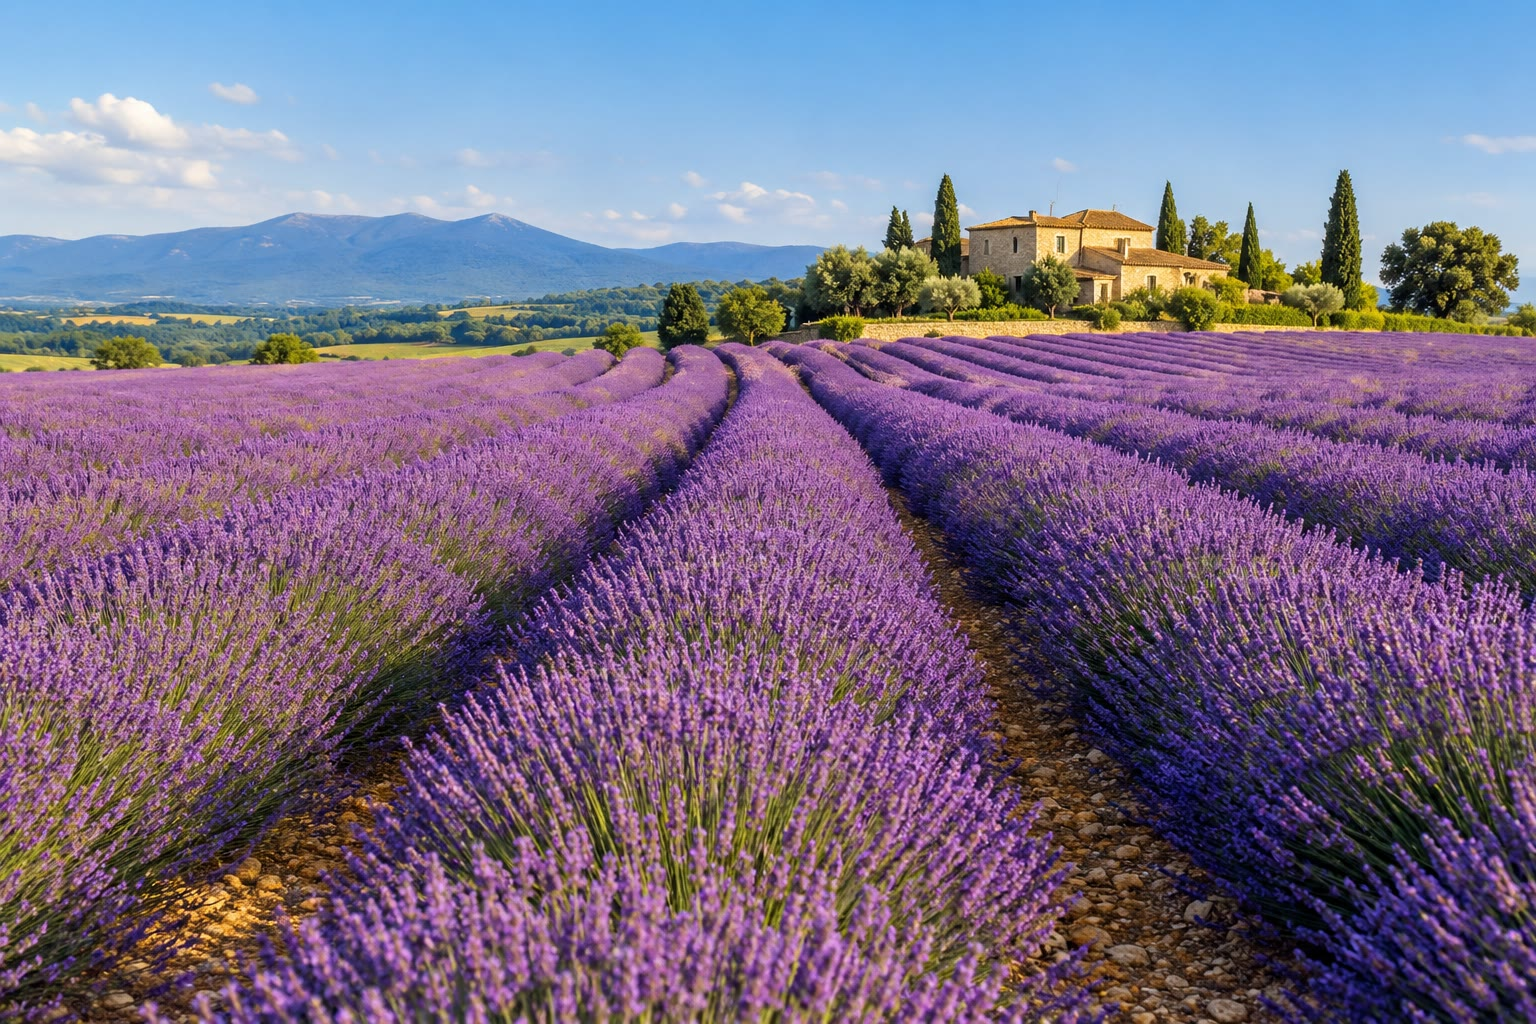
\includegraphics[width=0.55\linewidth]{images/book1/ai/g10-lavender-field.jpg}

{\small Um campo de lavanda em flor: a \omterm{def:g5:raw-materials-and-recycling:raw-material}{matéria-prima} do óleo essencial de
lavanda.}
\end{omfigure}

\section{Exercícios}

\begin{exercise}[$\star$]\label{exo:g10:chemical-species:1}
\omterm{def:g10:chemical-species:natural}{Espécie natural} ou sintética? A vanilina de uma vagem de baunilha; a
aspirina; a cafeína dos grãos de café; a vanilina produzida numa
fábrica.
\end{exercise}

\begin{exercise}[$\star$]\label{exo:g10:chemical-species:2}
Por que a vanilina sintética e a vanilina natural têm o mesmo ponto de
fusão?
\end{exercise}

\begin{exercise}[$\star$]\label{exo:g10:chemical-species:3}
Numa placa de CCD, a frente do \omterm{def:g6:solutions-and-solubility:solute}{solvente} está \qty{6.0}{cm} acima da
linha de partida e uma mancha está \qty{2.4}{cm} acima dela. Calcule o
$R_f$ dessa mancha.
\end{exercise}

\begin{exercise}[$\star$]\label{exo:g10:chemical-species:4}
Dê o papel do condensador numa \omterm{def:g10:chemical-species:distillation}{destilação}, e diga por que a água fria
entra pela extremidade de baixo.
\end{exercise}

\begin{exercise}[$\star$]\label{exo:g10:chemical-species:5}
Dê as três condições que um \omterm{def:g6:solutions-and-solubility:solute}{solvente} de \omterm{def:g10:chemical-species:extraction}{extração} deve cumprir.
\end{exercise}

\begin{exercise}[$\star\star$]\label{exo:g10:chemical-species:6}
Usando a tabela de \omterm{def:g6:solutions-and-solubility:solute}{solventes}, explique por que o etanol não pode ser
usado para extrair o linalol do destilado, enquanto o ciclo-hexano pode.
\end{exercise}

\begin{exercise}[$\star\star$]\label{exo:g10:chemical-species:7}
Num funil de separação, agita-se diclorometano com água. Que camada
fica em cima? Justifique com a tabela.
\end{exercise}

\begin{exercise}[$\star\star$]\label{exo:g10:chemical-species:8}
Um pó branco vendido como aspirina começa a fundir a \qty{126}{\celsius}
e está completamente fundido a \qty{132}{\celsius}. O que você pode
concluir?
\end{exercise}

\begin{exercise}[$\star\star$]\label{exo:g10:chemical-species:9}
Olhe a figura da CCD deste capítulo. O que o óleo de lavanda contém?
Que espécie subiu mais alto?
\end{exercise}

\begin{exercise}[$\star\star$]\label{exo:g10:chemical-species:10}
Ponha em ordem as etapas da obtenção do óleo de lavanda no laboratório:
separação das camadas; \omterm{def:g10:chemical-species:distillation}{hidrodestilação}; acréscimo de ciclo-hexano ao
destilado e agitação; \omterm{def:g3:separating-mixtures:evaporate}{evaporação} do ciclo-hexano.
\end{exercise}

\begin{exercise}[$\star\star$]\label{exo:g10:chemical-species:11}
Por que a linha de partida de uma placa de CCD é traçada a lápis e
colocada acima do \omterm{def:g10:chemical-species:tlc}{eluente}?
\end{exercise}

\begin{exercise}[$\star\star\star$]\label{exo:g10:chemical-species:12}
Depois da \omterm{def:g10:chemical-species:extraction}{extração}, o ciclo-hexano é retirado por um aquecimento suave,
e fica o óleo. Usando as temperaturas de ebulição do ciclo-hexano e do
linalol (\qty{198}{\celsius}), explique por que isso funciona.
\end{exercise}

\begin{exercise}[$\star\star\star$]\label{exo:g10:chemical-species:13}
Uma amostra sintética de um aroma dá uma única mancha numa placa de CCD,
na altura da \omterm{def:g10:chemical-species:natural}{espécie natural}, e funde de uma vez na temperatura certa.
Que duas conclusões você pode tirar?
\end{exercise}

\begin{exercise}[$\star\star\star$]\label{exo:g10:chemical-species:14}
Na mesma CCD, a mancha A tem $R_f = 0.40$ e a frente está \qty{5.5}{cm}
acima da linha. A que altura está a mancha A? Outra espécie tem
$R_f = 0.75$: a que distância acima da mancha A ela fica?
\end{exercise}

\begin{exercise}[$\star\star\star$]\label{exo:g10:chemical-species:15}
\qty{1.6}{g} de linalol podem se \omterm{def:g2:mixing-and-dissolving:dissolve}{dissolver} em \qty{1}{L} de água. Um
destilado de \qty{200}{mL} de água contém \qty{0.20}{g} de linalol
dissolvido. Ele está saturado? Quanto ele ainda poderia \omterm{def:g2:mixing-and-dissolving:dissolve}{dissolver}? Por
que vale a pena extrair essa água com ciclo-hexano em vez de jogá-la
fora?
\end{exercise}

\clearpage % mantém o título junto da caixa do problema (ele tinha ficado isolado no pé de uma página)
\section{Problema: o perfume da lavanda}

\begin{problem}[{Problema de fim de semana --- de um cesto de flores de
lavanda a algumas gotas de óleo essencial, controladas por cromatografia}]
\label{pb:g10:chemical-species:1}
% ledger: rho:cyclohexane, bp:cyclohexane, rho:CH2Cl2, bp:linalool, ghs:cyclohexane
Num laboratório escolar, \qty{100}{g} de flores frescas de lavanda são
hidrodestiladas com água. O destilado, turvo, é agitado com \qty{20}{mL}
de ciclo-hexano num funil de separação; a camada de ciclo-hexano é
guardada e secada, e o ciclo-hexano é \omterm{def:g3:separating-mixtures:evaporate}{evaporado} com um aquecimento
suave. O que fica é o óleo essencial de lavanda. Use a tabela de
\omterm{def:g6:solutions-and-solubility:solute}{solventes} deste capítulo.

\medskip
\noindent\textbf{Parte I --- A \omterm{def:g10:chemical-species:distillation}{hidrodestilação}.}
\begin{enumerate}
  \item Qual é o papel da água fervente numa \omterm{def:g10:chemical-species:distillation}{hidrodestilação}?
  \item Qual é o papel do condensador? Por onde a água fria entra nele?
  \item O destilado mostra uma fina camada oleosa flutuando sobre a água.
        O óleo é \omterm{def:g6:solutions-and-solubility:miscible}{miscível} com a água? Ele é mais ou menos denso que a
        água?
  \item Por que o destilado não é simplesmente despejado com cuidado para
        recuperar o óleo?
\end{enumerate}

\medskip
\noindent\textbf{Parte II --- A \omterm{def:g10:chemical-species:extraction}{extração}.}
\begin{enumerate}[resume]
  \item Por que o ciclo-hexano é um \omterm{def:g6:solutions-and-solubility:solute}{solvente} adequado para essa \omterm{def:g10:chemical-species:extraction}{extração}?
  \item O etanol poderia ser usado no lugar dele? Explique.
  \item Depois da agitação e do repouso, a camada de ciclo-hexano fica em
        cima ou embaixo? E com o diclorometano?
  \item Dê duas precauções exigidas pelos pictogramas do ciclo-hexano.
  \item Por que o ciclo-hexano pode ser \omterm{def:g3:separating-mixtures:evaporate}{evaporado} sem perder o linalol, que ferve a \qty{198}{\celsius}?
\end{enumerate}

\medskip
\noindent\textbf{Parte III --- A cromatografia.}
O óleo, o linalol puro (L) e o etanoato de linalila puro (A) são
aplicados numa placa de CCD. Depois da eluição, a frente está
\qty{6.0}{cm} acima da linha de partida. O óleo dá duas manchas, a
\qty{2.4}{cm} e a \qty{4.5}{cm}; a mancha L está a \qty{2.4}{cm}, a
mancha A a \qty{4.5}{cm}.
\begin{enumerate}[resume]
  \item Calcule o $R_f$ do linalol e o do etanoato de linalila.
  \item O que o óleo contém, até onde esta placa mostra?
  \item O óleo de lavanda é uma \omterm{def:g6:pure-substances-and-mixtures:pure-substance}{substância pura}?
  \item Por que as referências foram aplicadas na mesma placa que o óleo?
  \item Um linalol sintético é aplicado em outra placa, eluída nas mesmas
        condições: a mancha dele tem $R_f = 0.40$. O que se pode
        concluir?
\end{enumerate}

\medskip
\noindent\textbf{Parte IV --- Quanto óleo?}
O óleo obtido ocupa \qty{1.0}{mL}; \qty{1}{mL} desse óleo pesa
\qty{0.90}{g}.
\begin{enumerate}[resume]
  \item Que massa de óleo foi obtida?
  \item Que porcentagem da massa das flores é isso?
  \item Que massa de flores seria necessária para \qty{100}{g} de óleo?
  \item Diz-se que o óleo é ``natural''. Em que sentido isso é verdade? O
        linalol dele é diferente do linalol sintético?
  \item Dê a massa de óleo essencial obtida a partir de \qty{100}{g} de
        flores.
\end{enumerate}
\end{problem}
